
%%%%%%%%%%%%%%%%%%%%%%% file typeinst.tex %%%%%%%%%%%%%%%%%%%%%%%%%
%
% This is the LaTeX source for the instructions to authors using
% the LaTeX document class 'llncs.cls' for contributions to
% the Lecture Notes in Computer Sciences series.
% http://www.springer.com/lncs       Springer Heidelberg 2006/05/04
%
% It may be used as a template for your own input - copy it
% to a new file with a new name and use it as the basis
% for your article.
%
% NB: the document class 'llncs' has its own and detailed documentation, see
% ftp://ftp.springer.de/data/pubftp/pub/tex/latex/llncs/latex2e/llncsdoc.pdf
%
%%%%%%%%%%%%%%%%%%%%%%%%%%%%%%%%%%%%%%%%%%%%%%%%%%%%%%%%%%%%%%%%%%%


\documentclass[runningheads,a4paper]{llncs}

\usepackage{amssymb}
\setcounter{tocdepth}{3}
\usepackage{graphicx}
\usepackage[nolist]{acronym}

%\usepackage{hyphenat} see
%http://www.ctan.org/tex-archive/macros/latex/contrib/hyphenat - would
%be good to enable this to prevent hyphenation of OWL MS statements.
%Or find alternative

\usepackage{url}
\usepackage{tabularx}
\newcolumntype{Y}{>{\centering\arraybackslash}X}
\usepackage{makecell}
%\urldef{\mailsa}\path|davidos@ebi.ac.uk|

\newcommand{\keywords}[1]{\par\addvspace\baselineskip
\noindent\keywordname\enspace\ignorespaces#1}

\def\correspondingauthor{$^*$}
\def\@corresponding{\footnotesize\correspondingauthor Corresponding author} 


\begin{document}

\mainmatter  % start of an individual contribution

% first the title is needed
\title{Cell, chemical and anatomical views of the Gene Ontology: mapping to a Roche controlled vocabulary.}

% a short form should be given in case it is too long for the running head
\titlerunning{Cell, chemical and anatomical views of the Gene Ontology.}

% the name(s) of the author(s) follow(s) next
%
% NB: Chinese authors should write their first names(s) in front of
% their surnames. This ensures that the names appear correctly in
% the running heads and the author index.
%
\author{David Osumi-Sutherland$^1*$, Laura Badi$^2$, Enrico Ponta$^2$, Melanie Courtot$^1$ and Helen Parkinson$^1$}  % TBC

%
\authorrunning{Cell, chemical and anatomical views of the Gene Ontology.}
% (feature abused for this document to repeat the title also on left hand pages)

% the affiliations are given next; don't give your e-mail address
% unless you accept that it will be published
\institute{$^1$ European Bioinformatics Institute (EMBL-EBI), European Molecular Biology Laboratory, Wellcome Trust Genome Campus, Hinxton, Cambridge CB10 1SD, United Kingdom \\
$^2$ F. Hoffmann-La Roche Ltd
Grenzacherstrasse 124, CH-4070 Basel, Switzerland }
%* corresponding author: davidos@ebi.ac.uk

% \mailsa\\  % This needs to be fixed!

%
% NB: a more complex sample for affiliations and the mapping to the
% corresponding authors can be found in the file "llncs.dem"
% (search for the string "\mainmatter" where a contribution starts).
% "llncs.dem" accompanies the document class "llncs.cls".
%

\toctitle{}
\tocauthor{}
\maketitle


\begin{abstract}

The \ac{GO} is part of a network of logically interconnected ontologies including \ac{ChEBI}, the Cell Ontology and \ac{Uberon}.  These logical interconnections make it possible to query the \ac{GO} by cell type, chemical or anatomical structure, retrieving relevant \ac{GO} terms and associated annotations.  In this paper we describe the use of such queries to automate mappings from a controlled vocabulary developed by Roche to lists of terms from the \ac{GO}.

Using OWL-EL queries, we can fully automate mapping for about a third of terms in the Roche vocabulary, with another third having 5 or less \ac{GO} terms requiring manual mapping.

The approach we describe here is not limited to mapping external vocabularies on to the \ac{GO}. It could be used to provide chemical, cell or anatomically focussed ways of grouping \ac{GO} annotations and of performing enrichment analyses. It could also be used for more sophisticated, combinatorial queries of the \ac{GO} and its annotations.


\keywords{OWL, OWL-EL, controlled vocabulary}
\end{abstract}

\section{Introduction}


The \acf{GO} is widely used to annotate and group gene products according to their subcellular location (e.g., endoplasmic reticulum), molecular function (e.g., enzyme activity) and their wider role in cellular, developmental and physiological processes (e.g., signal transduction) {\cite{GO2015}). The logical structure of the ontology is used to group genes annotated with related terms and for term enrichment, a technique for determining the over- or under-representation of general classes of gene products in experimental datasets \cite{Shah2012}. Grouping and term enrichment typically only use logical relationships \textit{within} each of the 3 sub-ontologies of the \ac{GO} - cellular component, molecular function and biological process.
%
In recent years, \ac{GO} has switched its underlying formalization to Web Ontology Language (OWL2) (\url{http://www.w3.org/TR/owl2-primer/}), and has dramatically increased the number of logical axioms (Mungall et al., 2014). This new axiomatisation includes many new relationship types, relationships between terms in different \ac{GO} sub-ontologies and extensive logical links to terms from external ontologies including the cell ontology \cite{Meehan2011}, the chemical ontology ChEBI {\cite{Hastings2013} and the Uberon multi-species anatomy ontology \cite{Haendel2014}.  For example, the chemical participants in over 12,000 processes or functions are specified in the \ac{GO} via axioms referencing chemical entities defined by ChEBI \cite{Hill2013}. Over 8000 \ac{GO} classes have some direct or indirect logical link to a term from the Cell ontology or Uberon. These record, for example, the location of cellular components (e.g., the acrosome and its parts are present only in sperm), cell types that are the sole location of some process (e.g., 'natural killer cell degranulation' only occurs in natural killer cells ), and the products of developmental processes (e.g., bone is a product of 'bone morphogenesis').

Axiomatisation of the \ac{GO} is limited to the EL profile of OWL \cite{Mungall2014}. This allows \ac{GO} infrastructure to take advantage of fast, scalable OWL-EL reasoners such as ELK \cite{kazakov2012} to leverage the classifications in external ontologies to automate classification in \ac{GO}, and to ensure that classification and querying of the \ac{GO} will not become intractable as the ontology grows.  There is also great potential for using this axiomatisation to provide new, biologically meaningful systems for grouping annotations and term enrichment.  For example, we might want to group all annotations to genes involved in processes occurring in T-cells or in the pancreas, or to group annotations to genes involved in the processes involving nitric oxide.  In this paper we describe an implementation of this strategy in support of a use case from the pharmaceutical company Roche.

Roche uses a controlled vocabulary internally (from hereon referred to as RCV).  RCV consists of around 360 undefined terms, each of which is mapped to a set of terms from the \ac{GO}. RCV includes terms named for biological processes and, more rarely, for molecular functions and cellular components.  It also includes many terms named for types of cell, chemical, anatomical structure and taxonomic group. Prior to this work, mappings from RCV to the \ac{GO} were made manually, based on the lexical content of the names of \ac{GO} terms and the biological knowledge of those doing the mapping.  As the \ac{GO} evolved, it became increasingly impractical for Roche to keep this mapping complete and up-to-date via manual mapping.
%
Here we describe the development and testing of an automated mapping between \ac{GO} and RCV, making use of OWL-EL reasoning and a standard system for specifying OWL design patterns.


\section{Methods}

All code, mapping tables and results for the pipeline were maintained in a GitHub repository (\url{https://github.com/GO-ROCHE-COLLAB/Roche_CV_mapping}). As well as providing version control, Github allows nicely formatted display of mapping and results files in an easily editable form (tab separated value (TSV)), which can be easily edited via copying and pasting from excel spreadsheets. It also has an integrated ticket system, with an open API.  Standard mapping tickets were generated by script for all RCV terms mapped. A standard system of ticket labels allowed tracking of the approval status of all mappings.  The archived tickets constitute an audit trail for approval of mappings.
%
The mapping was specified using a single TSV file in which each line maps an RCV term to a mapping query and a term from \ac{GO}, ChEBI, CL, Uberon or NCBI taxonomy.
%
OWL reasoning was carried out via calls to a standard Java API for OWL using the ELK OWL reasoner \cite{kazakov2012}.  The query and processing pipeline was written in Jython, a Python implementation over Java (\url{http://www.jython.org/}).  %The pipeline produced a set of results tables, one for each RCV term, in TSV format.  These were used for review of mappings by Roche. 

\subsection{Mapping strategy}

In the manual mapping between RCV and \ac{GO} specified by Roche, multiple \ac{GO} terms are mapped to each RCV term. For the purposes of automated mapping, we interpret the mapped \ac{GO} terms as subclasses of the class referred to by the RCV term. For each RCV term, we attempted to find an equivalent class expression (a mapping query) that reflected the intended meaning of the RCV term, as judged by the RCV term name and manual mappings and based on discussion with Roche.
%
Mapping to fully expressive OWL-DL class expressions poses serious problems for scalability: querying and classification of the \ac{GO} with OWL-DL reasoners is already slow, and may become intractable as the \ac{GO} grows.  For this reason, we chose to restrict mappings to EL class expressions and use the fast, scaleable EL reasoner, ELK to run queries \cite{kazakov2012}. But this poses a problem for expressiveness: EL lacks various elements of OWL that are potentially useful for mapping queries - most notably disjunction (OR) and negation (NOT).  

To compensate partially for the lack of disjunction in OWL-EL, we developed a set of high level object properties for use in queries. For example, we define \textbf{occurs\_in\_OR\_has\_participant} as a grouping relation, allowing queries for processes that occur in a specified cell, or have that cell as a participant. Similarly, \ac{GO} does not use a reflexive relation for 'part of', but using one for query purposes means a query for subclasses of  ``'part of' some X" returns both subclasses and proper parts of class X.
%
Many RCV terms group processes in which a specified chemical or cell participates, with processes regulating those in which it participates (see Table 1 for example). To support such groupings, we used an OWL property chain axiom (\url{http://www.w3.org/TR/owl2-primer/#Property_Chains}) to define a relation, \textbf{regulates\_o\_has\_participant}, to query for processes that regulate a process in which some specified entity is a participant. We then define a super-property, \textbf{participant\_OR\_reg\_participant}, for this new relation and \textbf{has\_participant}

\begin{quote} % install /nohyphens for this?
\textbf{regulates} \textit{o} \textbf{has\_participant} \textit{subPropertyOf} \textbf{participant\_OR\_reg\_participant}

\textbf{regulates\_o\_has\_participant} \textit{subPropertyOf} \textbf{participant\_OR\_reg\_participant}

\textbf{has\_participant} \textit{subPropertyOf} \textbf{participant\_OR\_reg\_participant}
\end{quote}

In order to keep the mapping process simple, we added a further restriction: only a single mapping class was specified for each mapping.

The heavy use of OWL Object Property axioms to compensate for loss of expressivity tends to obscure the semantics of mappings. In order to communicate the meanings of mappings clearly, we used a script to generate human readable descriptions for each mapping query.  For example, we mapped the RCV term cannabinoid to the ChEBI term cannabinoid (CHEBI:67194) plus pattern \textbf{participant\_OR\_reg\_participant}.  The automated description of the mapping reads:  ``A process in which a cannabinoid participates, or that regulates a process in which a cannabinoid participates."

\begin{table}
 \caption{Example mapping table.}
      \label{tab:mapping}
      \begin{tabularx}{\textwidth}{@{}| c | c|Y|Y|Y|Y|Y|@{}}
        \hline
        \textbf{name}&\textbf{ID}&\textbf{manual}&\textbf{auto}&\textbf{checked}&\textbf{\thead{black\\listed}}&\textbf{\thead{is\\obsolete}} \\ \hline 
        \thead{regulation of \\ endocannabinoid \\ signaling pathway}&\ac{GO}\_2000124&1&1&1&0&0 \\ \hline
        \thead{cannabinoid \\signaling pathway}&\ac{GO}\_0038171&1&1&1&0&0 \\ \hline
        \thead{endocannabinoid \\signaling pathway}&\ac{GO}\_0071926&0&1&0&0&0 \\ \hline
        \thead{cannabinoid \\receptor activity}&\ac{GO}\_0004949&0&1&0&0&0 \\ \hline
       \thead{ cannabinoid \\biosynthetic process}&\ac{GO}\_1901696&0&1&0&0&0 \\ \hline
        \end{tabularx}
 \end{table}
 
Each mapping was used to generate a mapping table for manual review (an example is shown in table \ref{tab:mapping}), allowing the possibility of blacklisting either automated mappings or manual mappings (as a way of specifying corrections to the original manual mapping).



\section{Results}


 
We successfully mapped 308/364 RCV terms to mapping queries.  As shown in Table \ref{tab:summary_stats}, over a third (104) of the mapping queries were sufficient - meaning that no manual maintenance is required - and a further third of the mappings (148) had 10 or fewer additional manual mappings (Figure \ref{fig:man_only}).

  \begin{table}
 \caption{\textbf{Summary of mappings.}\textit{Auto sufficient:} Number of RCV terms for which no manual mapping required; \textit{Manual only}: Number of \ac{GO} terms only in manual mapping,  \textit{Auto only}: Number of \ac{GO} terms only in automated mapping; \textit{Manual blacklist} Number of blacklisted manually mapped terms; \textit{Auto blacklist}: blacklisted terms in automated mapping. Average and median values are per RCV term.}
\label{tab:summary_stats}
\centering
\begin{tabularx}{\textwidth}{@{}| c | Y|Y|Y|Y|Y|Y|@{}}
\hline
\thead{STAT}&\thead{RCV \\ name}&\thead{Auto \\ sufficient}&\thead{Manual \\ only}&\thead{Auto \\ only}&\thead{Manual \\blacklist}&\thead{Auto\\ blacklist} \\ \hline
SUM&308&104&4133&44012&81&70 \\ \hline
AVERAGE&-&-&13.42&142.9&0.26&0.23 \\ \hline
MEDIAN&&-&2.0&25.0&0.0&0.0 \\ \hline
\end{tabularx}
 \end{table}
 
 
\begin{figure}
\centering
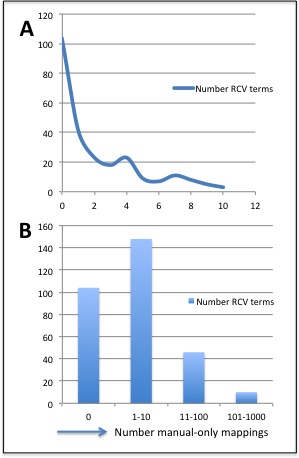
\includegraphics[width=70mm]{man_only.png}
\caption{\textbf{Distribution of manual only mappings.} A: Number of terms (Y-axis) vs number of manual mappings (X-axis) (cut-off at 20 manual mappings). 1B: Distribution of manual only mapping: 104 terms have no manual-mappings at all.  A further 148 have between 1 and 10.  The largest number of manual-only mappings for a single RCV terms was 323}
\label{fig:man_only}
\end{figure}
 
Mapping queries found many \ac{GO} terms that were not in the manual mapping, as shown on Figure \ref{fig:auto_only}.  For a few very general RCV classes (e.g., enzyme), over 1000 new mappings were found. Very few automated mappings were blacklisted - just 70 terms in total.  Blacklisting of terms ensured they were removed from the final mapping.

\begin{figure}
\centering
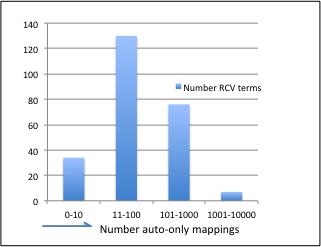
\includegraphics[width=70mm]{auto_only.png}
\caption{\textbf{Distribution of auto only mappings.}
X axis = number of auto-only mappings.  Y axis = Number of RCV terms.  Most mapping queries found under 100 additional (auto only) mappings, but over 75 found between 101 and 1000 and a few mapping queries found between 1001 and 10000 new mappings.}
\label{fig:auto_only}
\end{figure}

\section{Discussion and future directions}

This work demonstrates how the logical structure of the \ac{GO} can be used to achieve biologically meaningful mappings between \ac{GO} and terms from external controlled vocabularies or ontologies for which there is no corresponding \ac{GO} term.  For example, where the external vocabulary refers to a cell-type, a chemical or an anatomical structure.  The mapping system used is fast and scalable,  but a few improvements would be beneficial.

\subsection{Improving the RCV mapping pathway}




There is good scope for improving the mapping between RCV and \ac{GO} so that it is more thoroughly automated. As shown in Table \ref{mapping_patterns}, RCV term names follow patterns that mostly have consistent mappings patterns, but there are some exceptions.  More consistency in naming will make the meaning of terms more predictable and make the mapping of new terms more straightforward. 
\begin{table}
\caption{\textbf{Common mapping queries}}
\label{mapping_patterns}

\centering
%\begin{tabularx}{\textwidth}{@{}| Y | Y|Y|@{}}
\begin{tabularx}{\textwidth}{|
>{\centering\arraybackslash} X |
>{\centering\arraybackslash\advance\hsize2em }X |
>{\centering\arraybackslash}X |
}
\hline
 \thead{RCV term \\name pattern}& \thead{ Most common \\ mapping query \\(relation + target \\class ontology)}& \thead{No. cases different \\mapping query used} \\\hline
  chemical (e.g. cannabinoid)&participant\_OR\_reg\_participant + ChEBI (used 22 times)&7 \\\hline
  chemical metabolism &Equivalence + \ac{GO} (used 34 times)&6 \\\hline 
  cell type (e.g. T cell)&parts\_participation\_location + CL (covers parts, participant processes and processes occurring in cell type. used 30 times)&1 \\\hline
  X development (e.g. bone development)&is\_a\_OR\_part\_of\_OR\_regulates + \ac{GO} (used 41 times)&6 \\\hline
  X pathway/signalling (e.g. BMP signalling)&is\_a\_OR\_part\_of\_OR\_regulates + \ac{GO} (used 21 times)&6 \\\hline
\end{tabularx}
\end{table}

For RCV terms with only a small number of additional manual mappings, it may be worth considering whether the overhead of manual maintenance is worth the effort, especially where these additional mappings could not be achieved by further axiomatisation of the \ac{GO}.  For example, mappings to cell types often include mappings to growth factors acting on those cell types.  As these growth factors have much broader functions than action on the cell types for which they are named, \ac{GO} is unable to add any formal link between factors and cell types.

In other cases a mapping pattern involving two or more specified classes and a more sophisticated logic would be necessary to obtain a complete mapping.  For example, the manual mappings for X metabolism terms are consistently mapping to bot X metabolism and X transport terms in the \ac{GO}. A more complete mapping to RCV metabolism terms could be achieved using a pattern that named both \ac{GO} transport and \ac{GO} metabolic process terms.  This could be made scalable with a pathway that combines the results of multiple mapping patterns outside of OWL.

56 terms were not mapped.  Some were rejected from the pipeline as they were judged to be duplicates with other RCV terms.  The rest were rejected as currently unmappable due to the lack of suitable terms or axiomatisation within the \ac{GO} at this time.  For example, \ac{GO} currently has no way to group aerobic or anaerobic metabolic processes, although it does reflect the aerobic or anaerobic nature of many metabolic processes in their names and textual definitions. Further formalisation of the \ac{GO} is likely to improve the number of concepts that can be mapped.

\subsection{Alternative views of the \ac{GO} and its annotations}

The mechanisms described here for mapping to external ontologies could also be used for providing alternative views of the \ac{GO} and its annotations.  This is already reflected in some of the newer functionalities of the \ac{GO} browsing tool AMIGO, which now displayed inferred annotations to cell-types based on axioms in \ac{GO} recording where processes occur.  Figure \ref{fig:amigo} shows an AMIGO display of annotations to gene involved in processes occurring in T-Cells.


\begin{figure}
\centering
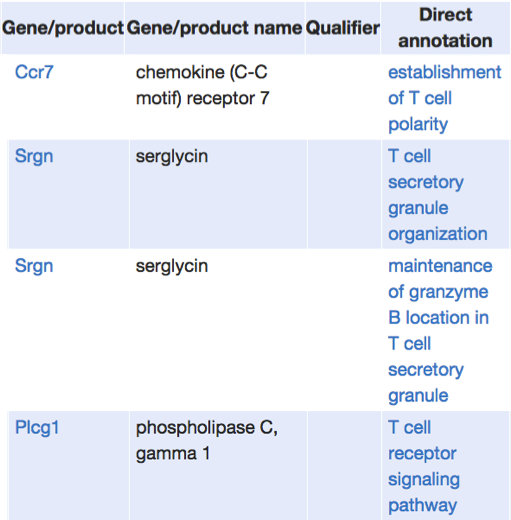
\includegraphics[scale=0.40]{amigo.png}
\caption{\textbf{The AmiGO \ac{GO} browsing tool displayes annotations to cells.}  The  T cell page on AmiGO displays annotations to processes that only occur in T-cells.  From http://amigo.geneontology.org/amigo/term/CL:0000084}
\label{fig:amigo}
\end{figure}

\subsection{Future work}

The system described here was designed to be lightweight and flexible, allowing maximum interaction between the designers of RCV at Roche and \ac{GO} editors with minimal development overhead.

The pattern-based system used here bears some relationship to the TermGenie system \cite{Dietze2014} which is already used to generate 80\% of new \ac{GO} terms.  One possible approach to fulfilling the needs of external groups for types of classification not included in the \ac{GO} would be to offer a TermGenie-like system for generating terms that group \ac{GO} terms in ways that are not currently supported internally by the \ac{GO}.



%
%\subsection*{Author's contributions}
%
%
%\subsection*{Acknowledgments.}
%Authors wish to acknowledge collaborators in the GO consortium.

\subsubsection*{Funding}

This work was supported by direct funding from F. Hoffmann-La Roche Ltd.  The Gene Ontology Consortium is supported by a P41 grant from the National Human Genome Research Institute (NHGRI) [grant 5U41HG002273-14].

%\begin{thebibliography}{}

\bibliography{Roche_swat4ls_2015} % Bibliography file (usually '*.bib' )

\bibliographystyle{plain}

%\end{thebibliography}

%%%%%%%%%%%


%%%%%%%%%%%%%%%%%%%%%%%%%%%%%%%%%%%
%%                               %%
%% Figures                       %%
%%                               %%
%% NB: this is for captions and  %%
%% Titles. All graphics must be  %%
%% submitted separately and NOT  %%
%% included in the Tex document  %%
%%                               %%
%%%%%%%%%%%%%%%%%%%%%%%%%%%%%%%%%%%

%%
%% Do not use \listoffigures as most will included as separate files










 



\begin{acronym}
\acro{OWL}{Web Ontology Language}
\acro{GO}{Gene Ontology}
\acro{OBI}{Ontology of Biomedical Investigations}
\acro{OBO}{Open Biomedical Ontologies}
\acro{BFO}{Basic Formal Ontology}
\acro{ChEBI}{Chemical Entities of Biological Interest}
\acro{Uberon}{Uber anatomy ontology}
\end{acronym}


\end{document}
